
\subsection{Longitudinal anisotropy}
\label{sec:psa:long}
Figure~\ref{fig:psa:vvse} shows the drift velocities along crystal axes as functions of electric field in [7,500]~V/mm. There is no transverse anisotropy of the drift along crystal axes. This figure is used to show the longitudinal difference of the drift velocity in different directions. 
\begin{figure}[tbhp]
  \centering
  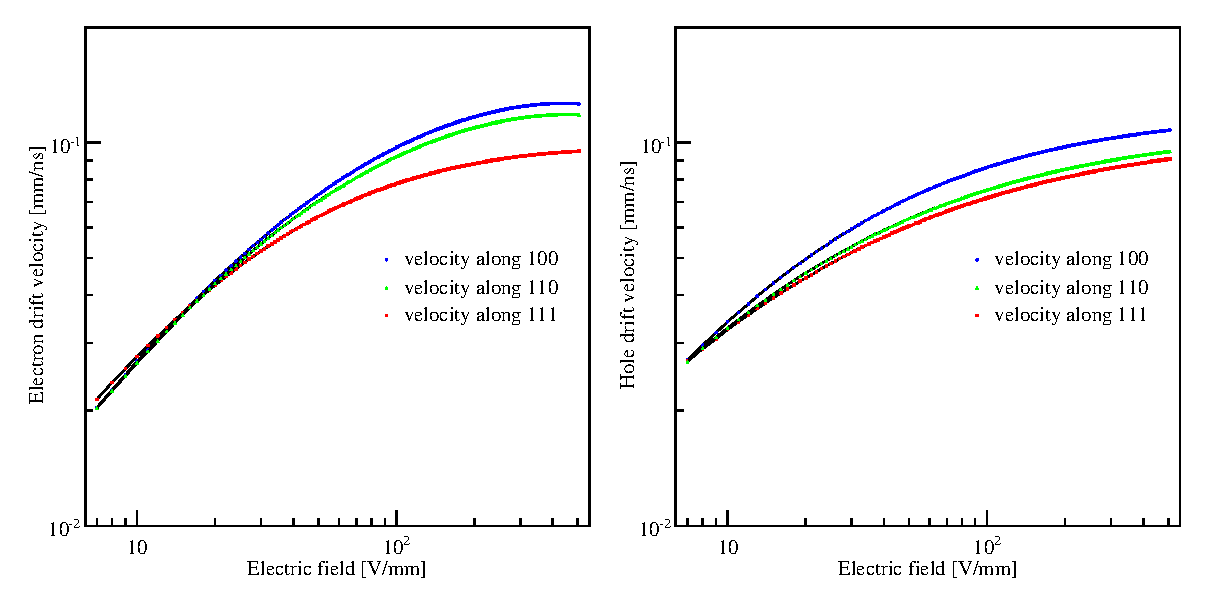
\includegraphics[width=\textwidth]{VvsElucian} \\\hfil
  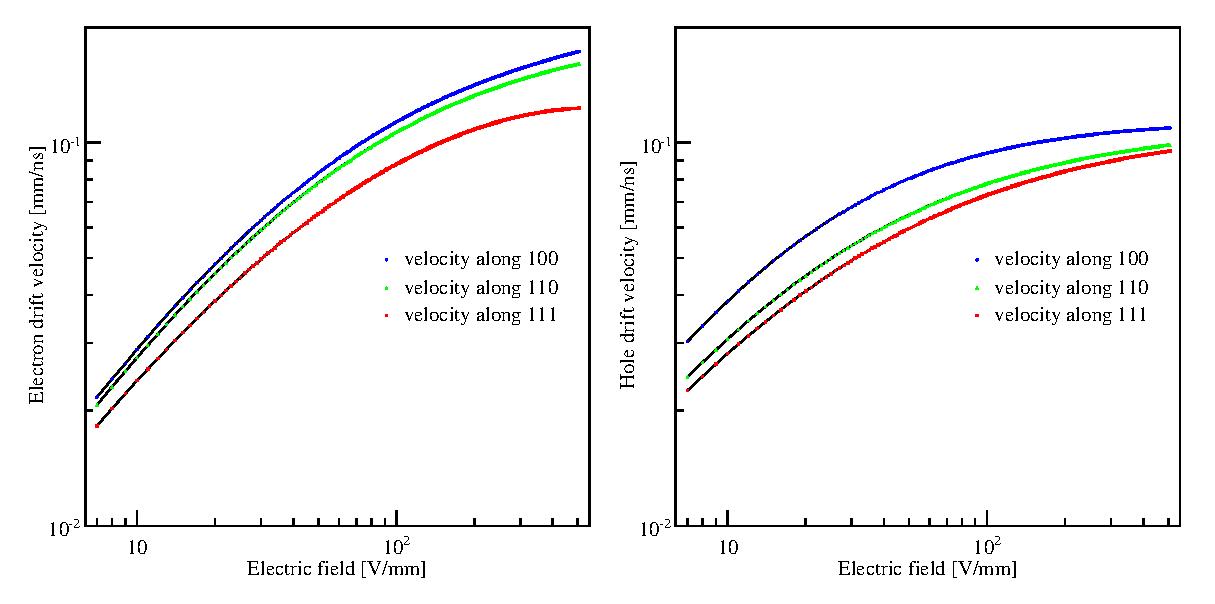
\includegraphics[width=\textwidth]{VvsEbart}
  \caption{Drift velocities along crystal axes as functions of electric field in [7,500]~V/mm. Velocities along crystal axes $\langle 100 \rangle$ and $\langle 111 \rangle$ are calculated with eq.~\ref{eq:pss:para}, while velocities along $\langle 110 \rangle$ are the simulated results. The upper plots are created using the input parameters provided in Ref.~\cite{miha}, the lower using the input parameters provided in Ref.~\cite{bart}.}
  \label{fig:psa:vvse}
\end{figure}

\subsection{Transverse anisotropy}
\label{sec:psa:tran}
Figure~\ref{fig:psa:trjs} shows the charge carrier drift trajectories on X-Y plane. The transverse anisotropy causes the bend of the trajectories. Also shown are the cross section of a true coaxial cylindrical germanium detector with inner radius of 5~mm and outer radius of 37.5~mm. The crystal axes are indicated with the signs $\langle 100 \rangle$, $\langle 110 \rangle$ and $\langle 010 \rangle$. The left plot shows the drift of electrons starting from the outer surface of the detector to the inside. The start points are distributed along the outer circle with equal distance between each other. The right plot shows the drift of holes starting from the inner surface to the outside. The start points are distributed along the inner circle with equal distance between each other. The applied high voltage is 3000~V. The time window is 400~ns. Within this time window all the electrons could reach the inner circle, while not all the holes could reach the outer circle.  This is because electrons drift slightly faster than holes, and along $\langle 110 \rangle$ direction holes drift slowest, as shown also in Fig.~\ref{fig:psa:vvse}.
\begin{figure}[tbhp]
  \centering
  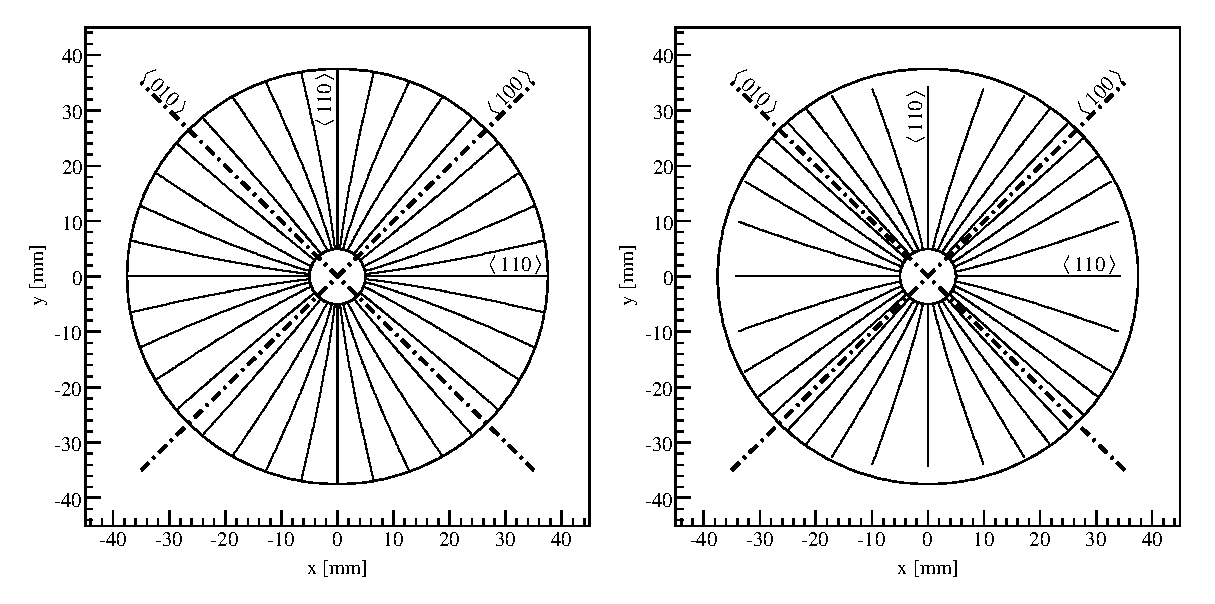
\includegraphics[width=\textwidth]{trjs}
  \caption{Charge carrier drift trajectories on X-Y plane. The     transverse anisotropy causes the bend of the trajectories. Also     shown are the cross section of a true coaxial cylindrical     germanium detector with inner radius of 5~mm and outer radius of     37.5~mm. The crystal axes are indicated with the signs $\langle     100 \rangle$, $\langle 110 \rangle$ and $\langle 010 \rangle$. The     left plot shows the drift of electrons starting from the outer     surface of the detector to the inside. The start points are     distributed along the outer circle with equal distance between     each other. The right plot shows the drift of holes starting from     the inner surface to the outside. The start points are distributed     along the inner circle with equal distance between each other. The     applied high voltage is 3000~V. The time window is 400~ns. Within     this time window all the electrons could reach the inner circle,     while not all the holes could reach the outer circle. This is     because electrons drift slightly faster than holes, and along     $\langle 110 \rangle$ direction holes drift slowest, as shown also     in Fig.~\ref{fig:psa:vvse}.}
  \label{fig:psa:trjs}
\end{figure}


%%% Local Variables:
%%% mode:latex
%%% TeX-master: "thesis"
%%% End:
